\chapter{Arithmetic Sequences and Series}

\section{General Formula}

\begin{proposition}\label{prop:arithmetic-general-formula}
	The general formula for an arithmetic sequence is given by:
	\begin{equation*}
		u_n = u_1 + (n-1)d
	\end{equation*}
	where $u_1$ is the first term, $d$ is the common difference, and $n$ is the term number.
\end{proposition}
\begin{proof}
We know that the first term is simply $u_1$. We obtain the second term by simply adding $d$ to the first term:
\begin{equation*}
	u_2 = u_1 + d
\end{equation*}
We employ a similar approach for the remaining terms:
\begin{align*}
	u_3 &= u_2 + d = u_1 + 2d \\
	u_4 &= u_3 + d = u_1 + 3d \\
	&\vdots \\
	u_n &= u_1 + (n-1)d
\end{align*}
\end{proof}

Determining the general formula of any arithmetic sequence is simply an exercise
in determining the first term and the common difference. This is not always straightforward.

\begin{exercise}
	An arithmetic sequence has third term $11$ and seventh term $23$. Find the general formula for this sequence.
\end{exercise}
\begin{answer}
	In this question, we are not given the first term of the common difference. We are told:
	\begin{align*}
		u_3 &= 11 \\
		u_7 &= 23
	\end{align*}
	Using the \hyperref[prop:arithmetic-general-formula]{general formula for arithmetic sequences}, we can express these terms in terms of $u_1$ and $d$:
	\begin{align*}
		u_3 &= u_1 + 2d = 11 \quad (1)\\
		u_7 &= u_1 + 6d = 23 \quad (2)
	\end{align*}
	Now, we must isolate and solve for $u_1$ and $d$. We can do this by subtracting equation (1) from equation (2):
	\begin{align*}
		(u_1 + 6d) - (u_1 + 2d) &= 23 - 11 \\
		4d &= 12 \\
		d &= 3
	\end{align*}
	We can now substitute this value of $d$ back into equation (1) to find $u_1$:
	\begin{align*}
		u_1 + 2(3) &= 11 \\
		u_1 + 6 &= 11 \\
		u_1 &= 5
	\end{align*}
	We find the general formula:
	\begin{equation*}
		u_n = 5 + (n-1)3 = 3n + 2
	\end{equation*}
\end{answer}

Finding the general formula for an arithmetic sequence is almost always a matter of
identifying the first term and the common difference, and then applying
\hyperref[prop:arithmetic-general-formula]{the general formula}. The above exercise shows you how 
to achieve this for more general questions.

\section{Arithmetic Series}

\begin{definition}[Arithmetic Series]\label{def:arithmetic_series}
	An \textit{arithmetic series} is the sum of the terms of an arithmetic sequence. If we take the first $n$ terms of an arithmetic sequence
	and add them together, we get a finite arithmetic series. Infinite arithmetic series are not considered, as they always diverge.
\end{definition}

\begin{remark}
	An arithmetic series can be represented using sigma notation, as the sum of the terms of an arithmetic sequence. 
	The sum of the first $n$ terms of an arithmetic sequence $\{u_n\}$ can be expressed as:
	\begin{equation*}
		S_n = \sum_{k=1}^{n} u_k
	\end{equation*}
	where $S_n$ is the sum of the first $n$ terms, and $u_k$ is the $k$th term of the arithmetic sequence.
\end{remark}

We will use the above to prove a useful formula for finding the sum of an arithmetic series, so it is important
that it makes sense. If it doesn't, try looking back over our discussion of \hyperref[sec:sigma-notation]{sigma notation}.

\begin{proposition}\label{prop:arithmetic-series-sum}
	The sum of the first $n$ terms of an arithmetic series is given by:
	\begin{equation*}
		S_n = \frac{n}{2}\left[2u_1 + (n-1)d\right]
	\end{equation*}
	where $u_1$ is the first term, $u_n$ is the $n$th term, and $n$ is the number of terms.
\end{proposition}
\begin{proof}
	First, we write our sum in sigma notation:
	\begin{equation}\label{eq:proof-2-1}
		S_n = \sum_{k=1}^{n} u_k
	\end{equation}
	We know that the $k$th term of an arithmetic sequence can be expressed as:
	\begin{equation*}
		u_k = u_1 + (k-1)d
	\end{equation*}
	Substituting this into equation \eqref{eq:proof-2-1}, we get:
	\begin{equation}\label{eq:proof-2-2}
		S_n = \sum_{k=1}^{n} \left[u_1 + (k-1)d\right]
	\end{equation}
	Remember, this is just a sum of terms, so we can split into two separate sums:
	\begin{equation}\label{eq:proof-2-3}
		S_n = \sum_{k=1}^{n} u_1 + \sum_{k=1}^{n} (k-1)d
	\end{equation}
	We can factor out the $d$ from the second sum, since it is constant with respect to $k$:
	\begin{equation}\label{eq:proof-2-4}
		S_n = \sum_{k=1}^{n} u_1 + d\sum_{k=1}^{n} (k-1)
	\end{equation}
	Notice that the second sum is now just $d$ times the sum of the first $n-1$ natural numbers. The sum of the
	first $m$ natural numbers is given by:
	\begin{equation*}
		\sum_{k=1}^{m} k = \frac{m(m+1)}{2}
	\end{equation*}
	(We won't prove this in these notes, but a proof can be found in the notes on `Proofs'). Using this 
	formula, we can express the second sum in equation \eqref{eq:proof-2-4} as:
	\begin{equation}\label{eq:proof-2-5}
		\sum_{k=1}^{n} (k-1) = \sum_{j=0}^{n-1} j = \frac{(n-1)n}{2}
	\end{equation}
	The first term in equation \eqref{eq:proof-2-4} is simply $n$ copies of $u_1$, since it is constant with respect to $k$, so
	we can express it as $u_1$ multiplied by $n$:
	\begin{equation}\label{eq:proof-2-6}
		\sum_{k=1}^{n} u_1 = nu_1
	\end{equation}
	Substituting equations \eqref{eq:proof-2-5} and \eqref{eq:proof-2-6} back into equation \eqref{eq:proof-2-4}, we get:
	\begin{align*}
		S_n &= nu_1 + d \cdot \frac{(n-1)n}{2} \\
		&= nu_1 + \frac{d(n-1)n}{2} \\
		&= \frac{2nu_1}{2} + \frac{d(n-1)n}{2} \\
		&= \frac{n}{2}\left[2u_1 + (n-1)d\right]
	\end{align*}
\end{proof}

\begin{remark}
	Notice that in the above proof, we could also have expressed the sum as:
	\begin{align*}
		S_n &= \frac{n}{2}(2u_1 + (n-1)d) \\
		&= \frac{n}{2}(u_1 + u_n)
	\end{align*}
	This is because $u_n = u_1 + (n-1)d$ by \hyperref[prop:arithmetic-general-formula]{the general formula for arithmetic sequences}.
\end{remark}

If the proofs above don't make immediate sense to you, they don't need to. In general, you won't need
to be able to understand the proof to use the formula, but it's often quite helpful to see where it comes from. 
Nonetheless, you are likely better served by a few worked examples. 

\newpage
\begin{exercise}[Easy]
	Bob arranges his books on a shelf such that the number of books on successive shelves forms an arithmetic sequence. If the first shelf has 20 books,
	and the fifth shelf has 44 books:
	\begin{enumerate}[label=(\alph*)]
		\item How many books are there on the
		\begin{tasks}[label=(\roman*)](1)
			\task 8th shelf?
			\task $n$th shelf?
		\end{tasks}
		\item Given that there are 12 shelves in total, how many books does Bob have?
	\end{enumerate}
\end{exercise}
\begin{answer}
	We are given:
	\begin{align*}
		u_1 &= 20 \\
		u_5 &= 44
	\end{align*}
	Using \hyperref[prop:arithmetic-general-formula]{the general formula for arithmetic sequences}, we can express $u_5$ in terms of $u_1$ and $d$:
	\begin{align*}
		u_5 = u_1 + 4d &= 44 \\
		20 + 4d &= 44 \\
		4d &= 24 \\
		d &= 6
	\end{align*}
	We can now find the required terms:
	\begin{enumerate}[label=(\alph*)]
		\item The number of books on:
		\begin{tasks}[label=(\roman*)](1)
			\task The 8th shelf:
			\begin{align*}
				u_8 &= u_1 + 7d \\
				&= 20 + 7(6) \\
				&= 62
			\end{align*}
			\task The $n$th shelf:
			\begin{align*}
				u_n &= u_1 + (n-1)d \\
				&= 20 + (n-1)(6) \\
				&= 6n + 14
			\end{align*}
		\end{tasks}
		\vspace{-20pt}
		\item The total number of books is the sum of the number of books on each shelf. Using \hyperref[prop:arithmetic-series-sum]{the formula for the sum of an arithmetic series}, we get:
		\begin{align*}
			S_{12} &= \frac{12}{2}[2(20) + (12-1)(6)] \\
			&= 6[40 + 66] \\
			&= 6(106) \\
			&= 636
		\end{align*}
	\end{enumerate}
\end{answer}

\newpage
\begin{exercise}[Medium]
	Alice is a student who loves reading books. By the end of her first week at school, she reads 1 book. By the end of her 
	fifth week, she reads 4 books. Assuming that the number of books she reads each week forms an arithmetic sequence, find:
	\begin{enumerate}[label=(\alph*)]
		\item The general formula for the number of books she reads in the $n$th week.
		\item The week in which Alice will read her 1000th book.
	\end{enumerate}
\end{exercise}
\begin{answer}
	We are given:
	\begin{align*}
		u_1 &= 1 \\
		u_5 &= 4
	\end{align*}
	Using \hyperref[prop:arithmetic-general-formula]{the general formula for arithmetic sequences}, we can express $u_5$ in terms of $u_1$ and $d$:
	\begin{align*}
		u_5 = u_1 + 4d &= 4 \\
		1 + 4d &= 4 \\
		4d &= 3 \\
		d &= \frac{3}{4}
	\end{align*}
	We can now find the required terms:
	\begin{enumerate}[label=(\alph*)]
		\item The general formula for the number of books she reads in the $n$th week:
		\begin{align*}
			u_n &= u_1 + (n-1)d \\
			&= 1 + (n-1)\left(\frac{3}{4}\right) \\
			&= \frac{3n - 3 + 4}{4} \\
			&= \frac{3n + 1}{4}
		\end{align*}
		\item To find the week in which Alice will read her 1000th book, we need to find the number of weeks that will
		have passed such that the total number of books read (i.e. the sum of the number of books read in each week up to that week)
		is equal to 1000. Hence, we set $S_n = 1000$ and solve for $n$ using \hyperref[prop:arithmetic-series-sum]{the formula for the sum of an arithmetic series}:
		\begin{equation*}
			S_n = \frac{n}{2}[2u_1 + (n-1)d] = 1000
		\end{equation*}
		Now, it is possible to solve this equation analytically (i.e. by hand), but it turns out to be much
		easier to solve this on your calculator. Simply set one equation equal to $y=1000$ and the other equal to $y=\frac{x}{2}[2(1) + (x-1)(\frac{3}{4})]$, where, in this case,
		$x$ represents $n$:
		% add the figure gdc-1 here
		\begin{figure}[H]
			\centering
			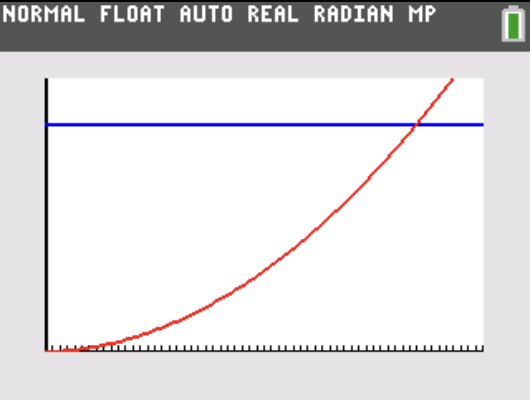
\includegraphics[width=0.4\textwidth]{Figures/gdc-1.png}
			\caption{Graphical solution to find the week in which Alice reads her 1000th book.}
			\label{fig:gdc-1}
		\end{figure}
	\end{enumerate}
	We can then use the intersect function on the calculator to find the value of $x$ (i.e. $n$)
	where the two lines meet. We find that $n \approx 57.4$. Since $n<57$, Alice will not have read her 1000th book
	by the end of week 57, but she will have by the end of week 58. Therefore, Alice will read her 1000th book in week 58.
\end{answer}

\begin{exercise}[Hard]
	Charlie sells math notes on the web. Each customer pays \$16.50 per month for access to all his notes. 
	By the end of the first month, he has 12 customers. By the end of the fourth month, he has 27 customers.
	Assuming that the number of customers he has each month forms an arithmetic sequence, how much revenue
	will Charlie have generated by the end of the first year?
\end{exercise}
\begin{answer}
	We are given:
	\begin{align*}
		u_1 &= 12 \\
		u_4 &= 27
	\end{align*}
	Using \hyperref[prop:arithmetic-general-formula]{the general formula for arithmetic sequences}, we can express $u_4$ in terms of $u_1$ and $d$:
	\begin{align*}
		u_4 = u_1 + 3d &= 27 \\
		12 + 3d &= 27 \\
		3d &= 15 \\
		d &= 5
	\end{align*}
	We now have a general formula for the number of customers paying Charlie in the $n$th month:
	\begin{align*}
		u_n &= u_1 + (n-1)d \\
		&= 12 + (n-1)(5) \\
		&= 5n + 7
	\end{align*}
	Thus, the revenue generated in the $n$th month is given by the product of the number of customers and the price:
	\begin{equation*}
		R_n = 16.50 \times u_n = 16.50(5n + 7) = 82.5n + 115.5
	\end{equation*}
	The monthly revenue also forms an arithmetic sequence, with first term $R_1 = 198$ and common difference $d_R = 82.5$.
	We can now use \hyperref[prop:arithmetic-series-sum]{the formula for the sum of an arithmetic series} to find the total revenue
	generated by the end of the first year (i.e. after 12 months):
	\begin{align*}
		S_{12} &= \frac{12}{2}[2(198) + (12-1)(82.5)] \\
		&= 6[396 + 907.5] \\
		&= 6(1303.5) \\
		&= 7821
	\end{align*}
	Thus, Charlie will have generated a total revenue of \$7821 by the end of the first year.
\end{answer}

\begin{exercises}[Arithmetic Sequences and Series]
\end{exercises}
\begin{questions}
  \begin{multicols}{2}
    \begin{enumerate}[label = \alph*), wide, leftmargin = *, itemsep = 1ex, after = \setcounter{enumi}{0}]
      \item Find the general formula for the following sequences:
      \begin{tasks}[label=\roman*)](1)
        \task $1, 3, 5, 7, 9, \ldots$
        \task $2, 6, 18, 54, 162, \ldots$
        \task $1, \frac{1}{4}, \frac{1}{9}, \frac{1}{16}, \ldots$
        \task $4, 9, 16, 25, 36, \ldots$
      \end{tasks}
      \vfill\null
      \columnbreak
      \item Task B
      \begin{tasks}(2)[label=\roman*]
      \task Item b1)
      \task Item b2)
      \task Item b3)
      \task Item b4)
      \end{tasks}
          \item Task C \begin{tasks}(2)
      \task Item b1)
      \task Item b2)
      \task Item b3)
      \task Item b4)
      \end{tasks}
    \end{enumerate}
  \end{multicols}
\end{questions}